\documentclass[12pt, a4paper]{article}
\usepackage{amsmath}
\usepackage{amsfonts}
\usepackage{amsthm}
\usepackage{mathtools}
\newtheorem{theorem}{Theorem}
\usepackage{pgfplots}
\pgfplotsset{width=10cm,compat=1.9}

\title{The beta distribution}
\author{Kristian Wichmann}

\begin{document}

\maketitle

The beta distribution is useful in a number of applications. Specifically, it is often used in Bayesian inference.

\section{Definition}
The pdf of the beta distribution has the interval $[0,1]$ as closed support. The pdf $f$ depends on two parameters, $\alpha$ and $\beta$:
\begin{equation}
\label{pdf1}
f(x)\propto x^{\alpha-1}(1-x)^{\beta-1}
\end{equation}
Here, the alpha indicates proportionality; there will also be a normalization constant that will depend on $\alpha$ and $\beta$:
\begin{equation}
\label{pdf2}
f(x)=\frac{1}{B(\alpha,\beta)} x^{\alpha-1}(1-x)^{\beta-1}
\end{equation}
Here, $B(\alpha,\beta)$ is known as the \textit{beta function}.

\section{The beta and gamma function relationship}
It turns out that the beta function can be expressed in terms of the gamma function, which is defined as
\begin{equation}
\label{gamma}
\Gamma(x)=\int_0^\infty e^{-u}u^{x-1}\ du
\end{equation}
To see this connection, consider the following expression:
\begin{align}
\Gamma(x)\Gamma(y)&=\int_0^\infty e^{-u}u^{x-1}\ du\int_0^\infty e^{-v}v^{y-1}\ dv\\
&=\int_0^\infty\int_0^\infty e^{-(u+v)}u^{x-1}v^{y-1}\ du\ dv
\end{align}
Now, consider the following change of variables:
\begin{equation}
(u,v)\mapsto(z,t),\quad u=zt,\quad v=z(1-t)
\end{equation}
Adding the definitions of the two new variables, we get $z=u+v$. From the first definition, we now get $t=\frac{u}{z}=\frac{u}{u+v}$. So $z$ can take on any value, but $t$ must be between 0 and 1. The corresponding Jacobian matrix is:
\begin{equation}
J=\begin{pmatrix}
\frac{\partial u}{\partial z}	& \frac{\partial v}{\partial z} \\
\frac{\partial u}{\partial t}	& \frac{\partial v}{\partial t} \\
\end{pmatrix}
=\begin{pmatrix}
t	& 1-t \\
z	& -z \\
\end{pmatrix}
\end{equation}
The determinant of $J$ is $t(-z)-z(1-t)=-z$, so $|\textrm{det}J|=z$. Now the integral reads:
\begin{equation}
\int_0^1\int_0^\infty e^{-z}(zt)^{x-1}(z(1-t))^{y-1}\cdot\underbrace{z}_{|\textrm{det}J|} dz\ dt
\end{equation}
Now rearrange to get:
\begin{equation}
\int_0^1 t^{x-1}(1-y)^{y-1}\ dt\int_0^\infty e^{-z}z^{x+y-1}\ dz=B(x,y)\Gamma(x+y)
\end{equation}
This means that:
\begin{equation}
\Gamma(x)\Gamma(y)=B(x,y)\Gamma(x+y)\Leftrightarrow B(x,y)=\frac{\Gamma(x)\Gamma(y)}{\Gamma(x+y)}
\end{equation}
In other words, the pdf for a beta distribution with parameters $\alpha$ and $\beta$ is:
\begin{equation}
\label{pdf3}
f(x)=\frac{\Gamma(\alpha+\beta)}{\Gamma(\alpha)\Gamma(\beta)} x^{\alpha-1}(1-x)^{\beta-1}
\end{equation}
A few of the possible pdf's are graphed below:

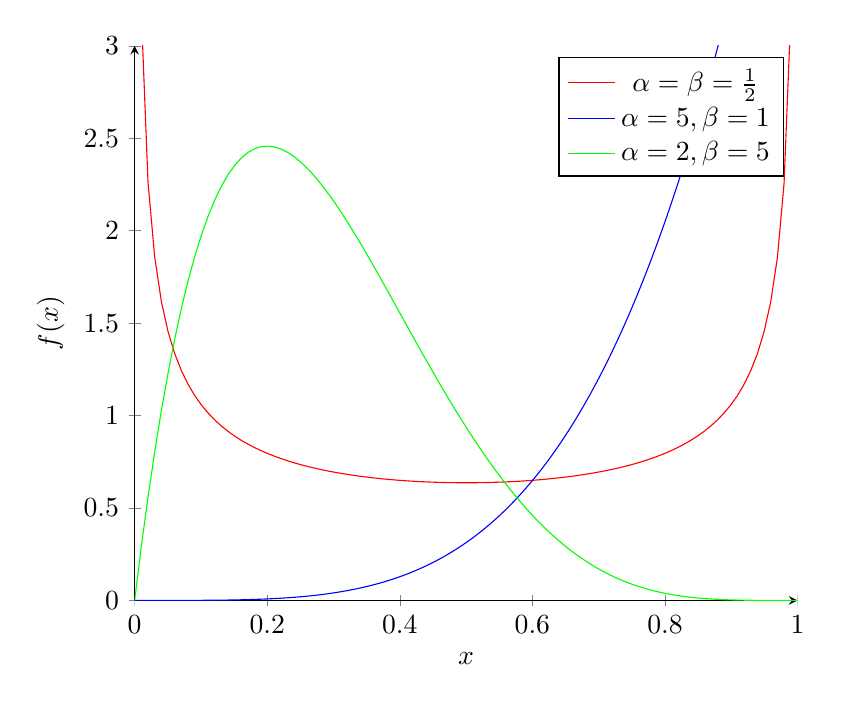
\begin{tikzpicture}
\begin{axis}[
    axis lines = left,
    xlabel = $x$,
    ylabel = {$f(x)$},
    ymin = 0,
    ymax = 3,
]
\addplot [
    domain=0:1, 
    samples=100, 
    color=red,
]
{1/3.14159265 * 1/x^0.5 * 1/(1-x)^0.5};
\addlegendentry{$\alpha=\beta=\frac{1}{2}$}
\addplot [
    domain=0:1, 
    samples=100, 
    color=blue,
    ]
    {5 * x^4};
\addlegendentry{$\alpha=5, \beta=1$}
\addplot [
    domain=0:1, 
    samples=100, 
    color=green,
    ]
    {30 * x * (1-x)^4};
\addlegendentry{$\alpha=2, \beta=5$}
 
\end{axis}
\end{tikzpicture}

\section{Moments}
Consider the raw $n$'th moment of a beta distribution with parameters $\alpha$ and $\beta$:
\begin{equation}
\mu_n=\int_0^1 x^n f(x)\ dx=\frac{\Gamma(\alpha+\beta)}{\Gamma(\alpha)\Gamma(\beta)}\int_0^1 x^n x^{\alpha-1}(1-x)^{\beta-1}
\end{equation}
But this integral is simply the reciprocal of the normalization constant for a beta distribution with parameters $\alpha'=\alpha+n$ and $\beta$. In other words, the moment is:
\begin{equation}
\mu_n=\frac{\Gamma(\alpha+\beta)}{\Gamma(\alpha)\Gamma(\beta)}\frac{\Gamma(\alpha+n)\Gamma(\beta)}{\Gamma(\alpha+\beta+n)}=\frac{\Gamma(\alpha+\beta)\Gamma(\alpha+n)}{\Gamma(\alpha)\Gamma(\alpha+\beta+n)}
\end{equation}

\subsection{Mean}
When $n=1$, this becomes:
\begin{equation}
\mu=\frac{\Gamma(\alpha+\beta)\Gamma(\alpha+1)}{\Gamma(\alpha)\Gamma(\alpha+\beta+1)}
\end{equation}
But we know that $\Gamma(x+1)=x\Gamma(x)$, so:
\begin{equation}
\mu=\frac{\Gamma(\alpha+\beta)\alpha\Gamma(\alpha)}{\Gamma(\alpha)(\alpha+\beta)\Gamma(\alpha+\beta)}=\frac{\alpha}{\alpha+\beta}
\end{equation}

\subsection{Second moment and variance}
When $n=2$, we get:
\begin{equation}
\mu_2=\frac{\Gamma(\alpha+\beta)\Gamma(\alpha+2)}{\Gamma(\alpha)\Gamma(\alpha+\beta+2)}
\end{equation}
Now use the functional equation twice:
\begin{equation}
\Gamma(x+2)=(x+1)\Gamma(x+1)=x(x+1)\Gamma(x)
\end{equation}
So the second, raw moment can be written:
\begin{equation}
\mu_2=\frac{\Gamma(\alpha+\beta)\alpha(\alpha+1)\Gamma(\alpha)}{\Gamma(\alpha)(\alpha+\beta)(\alpha+\beta+1)\Gamma(\alpha+\beta)}=\frac{\alpha(\alpha+1)}{(\alpha+\beta)(\alpha+\beta+1)}
\end{equation}
The variance is equal to $\mu_2-\mu^2$:
\begin{equation}
\sigma^2=\frac{\alpha(\alpha+1)}{(\alpha+\beta)(\alpha+\beta+1)}-\left(\frac{\alpha}{\alpha+\beta}\right)^2
\end{equation}
Getting a common denominator:
\begin{equation}
\sigma^2=\frac{\alpha(\alpha+1)(\alpha+\beta)-\alpha^2(\alpha+\beta+1)}{(\alpha+\beta)^2(\alpha+\beta+1)}
\end{equation}
Expand the numerator:
\begin{equation}
\alpha^3+\alpha^2\beta+\alpha^2+\alpha\beta-\alpha^3-\alpha^2\beta-\alpha^2=\alpha\beta
\end{equation}
So the variance is:
\begin{equation}
\sigma^2=\frac{\alpha\beta}{(\alpha+\beta)^2(\alpha+\beta+1)}
\end{equation}

\end{document}